% ============================================================
%  paper.tex
%  Decomposing the NL-to-Formal Proof Gap:
%  A Four-Layer Analysis of Why LLM Formal Theorem Proving
%  Stalls at 30-80%
%
%  Compile:  pdflatex paper.tex && bibtex paper && pdflatex paper.tex
%            && pdflatex paper.tex
% ============================================================
\documentclass[11pt,letterpaper]{article}

% ---------- Packages ----------
\usepackage[margin=1in]{geometry}
\usepackage{times}
\usepackage{amsmath,amssymb}
\usepackage{graphicx}
\usepackage{booktabs}
\usepackage{url}
\usepackage[hidelinks]{hyperref}
\usepackage{natbib}
\usepackage{tikz}
\usetikzlibrary{shapes.geometric,arrows.meta,positioning}
\usepackage{enumitem}
\setlist{itemsep=2pt,topsep=3pt}

% ---------- Bibliography ----------
\bibliographystyle{plainnat}

% ---------- Title ----------
\title{\bfseries From Natural Language to Formal Proof:\\
       An Intersemiotic-Translation Lens on the Reliability Gap
       in LLM Theorem Proving\vspace{-1ex}}

\author{Anonymous Author\\
        Challenge C2 Submission\\
        \today}

\date{}

% ============================================================
\begin{document}
\maketitle

% ---------- Abstract ----------
\begin{abstract}
\noindent
Translating a human-written mathematical proof into a formal language
such as Lean or Coq is, in Roman Jakobson's classic typology, an
\emph{intersemiotic translation}: an interpretation of one
sign system (informal mathematical English) by another (a typed
calculus with no tolerance for implicature). We adopt this lens to
re-examine a puzzling finding in neural theorem proving: state-of-the-art
provers on the standard \textsc{miniF2F} benchmark still reach only
$\approx$73\% pass@$k$, and DeepMind's silver-medal \textsc{AlphaProof}
at IMO~2024 relied on \emph{manually translated} problem statements.
We argue that end-to-end pass@$k$ figures are misleading because they
collapse four qualitatively distinct translation bottlenecks into a
single number. We decompose the gap into four layers---(L1) theorem
formalization, (L2) proof planning, (L3) low-level tactic detail, and
(L4) search and repair---and map published systems onto them. Read
through translation studies, these layers correspond to familiar
failure types: cultural/register untranslatability (L1), loss of
dynamic-equivalence cohesion (L2), collocational and grammatical errors
(L3), and iterative revision cycles (L4). Two findings stand out.
\emph{First}, L4 has been aggressively pushed by tree-search methods
(e.g.,~BFS-Prover at 72.95\%) but L1 remains essentially unsolved.
\emph{Second}, a Dafny back-end solves 40.6\% of \textsc{miniF2F}-test
with \emph{empty} proofs, a symbolic baseline almost no neural-proving
paper reports; the true LLM increment on the residual problems is
closer to 54\% than to 73\%. We propose a layer-resolved reporting
protocol and argue that the next breakthrough is more likely at L1/L2
than from further L4 search engineering.
\end{abstract}

% ============================================================
\section{Introduction}
\label{sec:intro}
% ============================================================

Large language models (LLMs) now write fluent natural-language (NL)
mathematical reasoning, but such reasoning is unverifiable: a coherent
chain-of-thought may contain an algebraic slip, a wrong lemma, or a
fabricated citation, and the reader---human or automated---has no
deterministic way to certify correctness
\cite{mao2024champ,frieder2023ghosts,collins2023checkmate}. Formal theorem proving (FTP)
offers the opposite trade-off: languages such as Lean, Coq, Isabelle/HOL,
and Dafny require every step to type-check, and the proof assistant
itself becomes a deterministic auditor. If an LLM can emit a proof
the assistant accepts, the result is, modulo the trusted kernel,
\emph{certified correct}.

This promise has driven a fast-moving sub-field. Yet the headline
numbers are puzzling. On \textsc{miniF2F}-test, the de facto
cross-assistant benchmark, GPT-4 zero-shot reaches 25.4\%
\cite{wang2024theoremllama}, fine-tuned open models reach
33.6\% \cite{wang2024theoremllama}, and ByteDance's BFS-Prover in 2025
sets the state of the art at 72.95\% pass@$k$ \cite{xin2025bfsprover}.
Even DeepMind's silver-medal system at IMO~2024 combined
\textsc{AlphaGeometry2} \cite{chervonyi2025alphageometry2} with
\textsc{AlphaProof} for algebra and number theory, and, as
\citet{jana2025proofbridge} explicitly note, \emph{problem statements
were manually translated} before automated proof synthesis began.
Why, after two years of rapid progress, does an IMO-level system still
need a human in the loop at the very first step?

We argue that the community's metric---end-to-end pass@$k$---is hiding
the answer. A 73\% pass rate on \textsc{miniF2F} could mean that
systems fail at four equally sized 27\% layers, or that they fail
exclusively on one hard layer while the other three are nearly solved.
These two diagnoses imply completely different research agendas.

We read this pipeline through a lens familiar in translation studies
and intercultural communication: following Jakobson's tripartite
typology, moving from informal mathematical English to a typed formal
calculus is an \emph{intersemiotic translation}---an interpretation of
one sign system by another \cite{jakobson1959translation}. Viewed this
way, the four bottlenecks below are not merely engineering problems;
they map onto well-understood categories of translation failure:
cultural/register untranslatability, loss of dynamic-equivalence
cohesion, collocational and grammatical error, and iterative revision.
This lens is not decorative: it explains why L1 (the most
``translation-like'' layer) is the least engineered, and why purely
engineering fixes (L4 search) have hit a ceiling rather than cracking
the problem.

\paragraph{Contributions.}
\begin{enumerate}[leftmargin=*]
  \item We decompose the NL-to-FL proof gap into four layers:
        \textbf{L1} theorem formalization (NL statement $\to$ FL
        statement), \textbf{L2} proof planning (high-level strategy
        decomposition), \textbf{L3} low-level tactic detail
        (unification, typeclass inference, rewrite direction), and
        \textbf{L4} search and repair (state-space exploration,
        compiler-feedback repair).
  \item We map twelve published systems onto this decomposition and
        show that current effort is heavily concentrated on L4, while
        L1 is almost untouched outside specialised neuro-symbolic
        engines.
  \item We highlight a baseline that is rarely reported: Dafny's
        empty-proof automation solves 40.6\% of \textsc{miniF2F}-test
        \cite{baksys2025mini2f2dafny}. Against this baseline the true
        LLM increment on the residual problems is $\approx$54\%, not
        73\%.
  \item We propose a layer-resolved evaluation protocol that makes the
        next research agenda diagnosable.
\end{enumerate}

% ============================================================
\section{Background}
\label{sec:bg}
% ============================================================

\paragraph{Proof assistants.}
Lean~4 has become the dominant platform for neural theorem proving,
largely because of the \textsc{Mathlib} mathematical library and the
LeanDojo environment \cite{song2024leancopilot}. Coq and Isabelle/HOL
have longer histories and larger software-verification user bases;
Dafny is unusual in that it ships with automated back-ends (SMT
solvers) that can discharge goals without any user-written tactic.
We refer to recent surveys for the broader landscape
\cite{lu2023survey,meadows2023mathnlp}.

\paragraph{Benchmarks.}
\textsc{miniF2F} is a cross-assistant benchmark of 244 test and 244
validation undergraduate-level problems, formalised in Lean,
Isabelle, HOL Light, and Metamath. \textsc{ProofNet}, \textsc{TRIGO}
\cite{xiong2023trigo}, and the Open Bootstrapped Theorems (OBT)
\cite{wang2024theoremllama} extend coverage to informal-proof
alignment and to symbolic simplification. We focus on \textsc{miniF2F}
because it is the only benchmark for which nearly every system reports
a comparable number.

\paragraph{Pipeline paradigms.}
Three paradigms dominate. \emph{Whole-proof generation} prompts the
LLM for a complete proof document in one shot (Baldur for Isabelle;
the Coq whole-proof line studied by \cite{prasad2024coq}).
\emph{Tactic prediction} feeds the current proof state to the LLM and
asks for the next tactic, iteratively; Lean Copilot
\cite{song2024leancopilot} is the canonical framework. \emph{Tree
search} wraps tactic prediction with a search algorithm (MCTS,
best-first search, or DPO-refined expansion) that explores multiple
proof states; BFS-Prover \cite{xin2025bfsprover} is the current
standard-bearer.

% ============================================================
\section{The Four-Layer Gap}
\label{sec:layers}
% ============================================================

We posit that an end-to-end NL-to-FL proof pipeline can fail at four
qualitatively distinct stages. Figure~\ref{fig:pyramid} summarises the
decomposition; we discuss each layer with evidence from published
error analyses.

\begin{figure}[t]
\centering
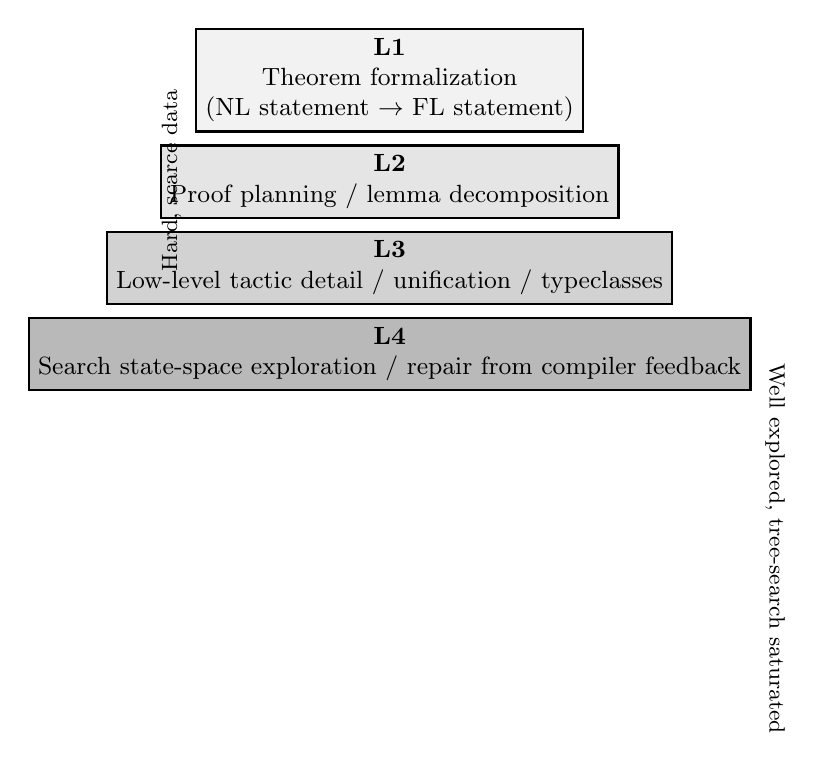
\begin{tikzpicture}[scale=1.0, every node/.style={align=center,font=\small}]
  \node[draw, thick, fill=gray!10, minimum width=3.2cm, minimum height=0.8cm] (L1)
        {\textbf{L1}\\ Theorem formalization\\ (NL statement $\to$ FL statement)};
  \node[draw, thick, fill=gray!20, minimum width=5.0cm, minimum height=0.8cm, below=0.15cm of L1] (L2)
        {\textbf{L2}\\ Proof planning / lemma decomposition};
  \node[draw, thick, fill=gray!35, minimum width=6.8cm, minimum height=0.8cm, below=0.15cm of L2] (L3)
        {\textbf{L3}\\ Low-level tactic detail / unification / typeclasses};
  \node[draw, thick, fill=gray!55, minimum width=8.6cm, minimum height=0.8cm, below=0.15cm of L3] (L4)
        {\textbf{L4}\\ Search state-space exploration / repair from compiler feedback};
  \node[left=0.3cm of L1, font=\footnotesize, rotate=90, align=center] {Hard, scarce data};
  \node[right=0.3cm of L4, font=\footnotesize, rotate=-90, align=center] {Well explored, tree-search saturated};
\end{tikzpicture}
\caption{The four-layer decomposition of the NL-to-FL proof gap.
Failure at a higher layer forces a human-in-the-loop step; failure at
L4 is the layer most systems currently engineer.}
\label{fig:pyramid}
\end{figure}

\subsection{L1: Theorem Formalization Gap}
\label{sec:l1}

\emph{Input:} a problem written for humans (e.g., an IMO statement in
English). \emph{Output:} a well-typed FL theorem that captures exactly
the intended mathematical content, including implicit domains,
variable types, and definitions drawn from the right library.

This layer is the least studied. \citet{jana2025proofbridge}
explicitly motivate ProofBridge by observing that \textsc{AlphaProof}'s
silver-medal IMO result required human translation of problem
statements. The challenge is not mere parsing: an NL statement like
``$f$ is continuous'' may require choosing between
\texttt{ContinuousMap}, \texttt{ContinuousOn}, and the topological
definition depending on context, and the wrong choice makes downstream
proof search fail for reasons that have nothing to do with the proof
itself.

ProofBridge attacks L1 with a joint NL--FL embedding and retrieval-
augmented fine-tuning, reporting a $+$31.14\% semantic-correctness gain
over a Kimina-Prover baseline on their curated \textsc{miniF2F}-Test-PF
split \cite{jana2025proofbridge}. \textsc{AlphaGeometry2}
\cite{chervonyi2025alphageometry2} covers 88\% of IMO 2000--2024
geometry statements with its own controlled input language, an
extension of the original AlphaGeometry's neuro-symbolic pipeline
\cite{trinh2023alphageometry}; but this coverage is achieved by
restricting the input language---precisely the manual formalization
step we identify as L1.

\paragraph{Translational reading.}
This layer is closest to what translation studies call \emph{cultural
untranslatability}: an NL statement draws on shared presuppositions of
the mathematics discourse community \cite{swales1990genre}---what
``continuous'' means in context, which library definition is
intended---that have no one-to-one formal counterpart. Venuti's
notion of \emph{domestication versus foreignization}
\cite{venuti1995invisibility} captures the design choice:
\textsc{AlphaGeometry2} ``domesticates'' by restricting the input
language, while ProofBridge attempts ``foreignization'' by accepting
raw NL. The modest $+$31\% semantic-correctness gain suggests that
foreignization is still brittle.

\subsection{L2: Proof Planning Gap}
\label{sec:l2}

\emph{Input:} a formal theorem statement. \emph{Output:} a sound
high-level decomposition into lemmas or sub-goals, without filling in
the low-level justifications.

Evidence that LLMs are weak at this layer comes from controlled
synthetic experiments. \citet{saparov2023prontoqa} parse generated
chain-of-thought into symbolic proofs in ProntoQA and find that models
produce \emph{individually correct deduction steps} but fail at
\emph{proof planning}: when multiple valid deductions are available,
they do not systematically explore alternatives and converge on
shallow, often dead-end paths. \citet{opedal2024mathgap} extend this
finding by generating problems with arbitrarily deep/wide proof trees
and showing performance degrades markedly as proof depth grows.

BC-Prover \cite{he2024bcprover} is a direct response: it introduces
``pseudo-steps'' that decompose the proof into backward-chained
sub-goals \emph{before} generating formal tactics, and reports
significant \textsc{miniF2F} gains. The very need for such a module
confirms that vanilla tactic prediction leaves L2 unaddressed.

\paragraph{Translational reading.}
In Nida's classic distinction \cite{nida1964science}, NL proofs strive
for \emph{dynamic equivalence}: a reader understands the intended
argument via connectives such as ``it remains to show that'' that elide
routine steps. Formal proofs instead require \emph{formal equivalence}
at every step. The L2 failure is precisely the loss of cohesion when
dynamic-equivalence connectives are stripped: the model knows the
destination but cannot map NL discourse markers onto a valid sub-goal
tree. This is why BC-Prover's ``pseudo-steps'' work---they reintroduce
an explicit discourse planner that the LLM otherwise omits.

\subsection{L3: Low-Level Tactic Detail Gap}
\label{sec:l3}

\emph{Input:} a proof state and a desired high-level step.
\emph{Output:} a well-typed tactic invocation with the right arguments,
typeclass instances, rewrites, and implicit parameters.

This is the layer where error analysis is richest.
\citet{lu2024palm} analysed 520 GPT-3.5 proof-generation errors in
Coq and found a strikingly consistent pattern: the model \emph{identified
the correct high-level structure} of the proof but failed on low-level
details (wrong unification, missing arguments, incorrect rewrite
direction). Their PALM system generates a proof then applies targeted
symbolic repairs to low-level failures, improving over baselines by
76.5\%--180.4\% across more than 10K theorems.

APRIL \cite{wang2026april} operationalises the same insight for Lean:
it constructs a 260K-tuple dataset of erroneous proofs paired with
compiler diagnostics and aligned repairs, and shows that a fine-tuned
4B model beats stronger open-source baselines on single-shot repair.
Both systems treat L3 as a feedback-driven repair problem rather than a
one-shot generation problem.

\paragraph{Translational reading.}
These are \emph{collocational and grammatical errors}: the equivalent
of a translator who chooses the right word but pairs it with the wrong
preposition, tense, or case. The LLM ``speaks'' the formal language at
the level of register \cite{swales1990genre} but violates its
selectional restrictions---which arguments a tactic expects, in which
order, with which implicit instance. APRIL's compiler-feedback loop is
analogous to a translator revising against native-speaker annotations:
a correction mechanism that presupposes the error has already happened,
rather than preventing it.

\subsection{L4: Search and Repair Gap}
\label{sec:l4}

\emph{Input:} an initial proof state. \emph{Output:} a path to a
closed state, allowing backtracking and intermediate repairs.

This is the layer that has seen the most engineering investment.
BFS-Prover \cite{xin2025bfsprover} reports 72.95\% on
\textsc{miniF2F}-test using best-first tree search with DPO on
compiler-error-annotated state--tactic pairs. The Coq whole-proof
line of \citet{prasad2024coq} lifts GPT-4 from 66.44\% to 79.42\% by
recursively extracting lemmas at failure points---a search strategy.
Lean Copilot \cite{song2024leancopilot} automates 74.2\% of proof
steps in the \textsc{Mathematics in Lean} textbook, an 85\% gain over
rule-based Aesop.

We read these numbers as evidence that L4 is approaching a local
ceiling given current LLM tactic-prediction quality: further gains
from better search alone appear to be incremental, not transformational.

\paragraph{Translational reading.}
This layer is the \emph{revision cycle} of professional translation:
draft, consult parallel texts, backtrack, try again. BFS-Prover and the
Coq lemma-extraction loop are industrial-scale versions of the
translator's draft-and-revise workflow. That L4 is the most engineered
layer makes sense---it is the one both translators and their
computer-aided translation tools already know how to optimise. It is
also, as the 72.95\% ceiling suggests, the layer where further
investment yields diminishing returns: better search cannot fix a
proof whose L1 formalization was wrong or whose L2 plan was ill-chosen.

% ============================================================
\section{Evidence Mapping}
\label{sec:mapping}
% ============================================================

Table~\ref{tab:systems} places representative systems on the four
layers. ``$\checkmark$'' denotes an explicit module addressing that
layer; ``$\sim$'' denotes incidental or partial treatment; ``--''
denotes no targeted mechanism.

\begin{table*}[t]
\centering
\small
\begin{tabular}{llccccc}
\toprule
System & Year & L1 & L2 & L3 & L4 & \textsc{miniF2F}-test \\
\midrule
GPT-4 zero-shot (FL theorem) & 2023 & -- & $\sim$ & $\sim$ & -- & 25.4\% \\
TheoremLlama \cite{wang2024theoremllama} & 2024 & bootstrapped & $\sim$ & $\checkmark$ & -- & 33.6\% \\
Lean Copilot \cite{song2024leancopilot} & 2024 & -- & $\checkmark$ & $\checkmark$ & -- & n/a (step-level) \\
PALM \cite{lu2024palm} & 2024 & -- & $\sim$ & $\checkmark$ (repair) & $\sim$ & $+$76--180\%$^\dagger$ \\
BC-Prover \cite{he2024bcprover} & 2024 & -- & $\checkmark$ (pseudo-steps) & $\sim$ & $\checkmark$ & SOTA at time \\
BFS-Prover \cite{xin2025bfsprover} & 2025 & -- & $\sim$ & $\sim$ & $\checkmark$ (DPO+BFS) & \textbf{72.95\%} \\
ProofBridge \cite{jana2025proofbridge} & 2025 & $\checkmark$ (joint emb.) & $\sim$ & $\checkmark$ & $\checkmark$ (repair) & +31.1\% SC$^\ddagger$ \\
\midrule
Dafny empty-proof \cite{baksys2025mini2f2dafny} & 2025 & n/a & n/a & n/a & SMT & \textbf{40.6\%} \\
\bottomrule
\multicolumn{7}{l}{\footnotesize $^\dagger$ Relative improvement over baselines on a $>$10K-theorem Coq corpus, not \textsc{miniF2F}.}\\
\multicolumn{7}{l}{\footnotesize $^\ddagger$ Semantic-correctness gain on the curated \textsc{miniF2F}-Test-PF split.}
\end{tabular}
\caption{Systems mapped onto the four layers. L4 is the most densely
addressed layer; L1 is addressed only by ProofBridge and the
geometry-specific \textsc{AlphaGeometry2} input language. The bottom
row is the symbolic baseline that almost no LTP paper reports.}
\label{tab:systems}
\end{table*}

Two observations follow.

\textbf{First, L4 is saturated; L1 is open.} Seven of eight neural
systems have an L4 component, but only ProofBridge explicitly
addresses L1, and even ProofBridge assumes the NL theorem is available
and focuses on translating it. No system in Table~\ref{tab:systems}
fully automates the path from an arbitrary olympiad NL statement to a
formalised theorem \emph{and} a verified proof. This is consistent
with the manual-translation caveat attached to \textsc{AlphaProof}.

\textbf{Second, improvements are cumulative, not compositional.}
BFS-Prover's 72.95\% is built on better L4 search but does not fix L3
root causes; PALM's 76--180\% L3 repair does not ship with an L2
planner. A system that stacked L1 (ProofBridge) + L2 (BC-Prover
pseudo-steps) + L3 (PALM/APRIL repair) + L4 (BFS search) has not, to
our knowledge, been published.

% ============================================================
\section{The Baseline Nobody Reports}
\label{sec:baseline}
% ============================================================

\textsc{miniF2F}-Dafny \cite{baksys2025mini2f2dafny} reports that
Dafny's built-in SMT automation discharges 99/244 (40.6\%) of the
\emph{test} set and 109/244 (44.7\%) of the validation set with
\emph{empty proofs}---no LLM, no tactic, no hint. For the residual
problems, the best off-the-shelf LLM reaches 55.7\% pass@4 with
iterative error correction.

This reframes the headline number. Let $p_{\mathrm{LLM}}=0.7295$ be
BFS-Prover's pass rate and $p_{\mathrm{SMT}}=0.406$ be the empty-proof
Dafny rate. The LLM's \emph{incremental} contribution on the problems
that symbolic automation cannot solve is

\begin{equation}
  \Delta_{\mathrm{LLM}}
  = \frac{p_{\mathrm{LLM}} - p_{\mathrm{SMT}}}
         {1 - p_{\mathrm{SMT}}}
  = \frac{0.7295 - 0.406}{1 - 0.406}
  \approx 0.543.
  \label{eq:delta}
\end{equation}

In other words, the LLM closes about 54\% of the residual gap, not
73\% of the total benchmark. We do not claim that BFS-Prover and Dafny
are directly comparable (they target different proof assistants and
different automation layers), but the methodological point stands:
\emph{any neural-proving result should be reported alongside the
performance of a symbolic-only baseline on the same problems}.
Without this, a 73\% figure can look twice as impressive as the
underlying LLM increment justifies.

% ============================================================
\section{Toward Layer-Resolved Evaluation}
\label{sec:protocol}
% ============================================================

We propose that future neural theorem-proving papers report, in
addition to end-to-end pass@$k$, the following per-layer quantities:

\begin{itemize}[leftmargin=*]
  \item $p_1$: fraction of NL statements automatically formalised
        with \emph{semantic equivalence} verified by proving the
        bidirectional implication of the NL-intended and FL statements
        (the metric ProofBridge already uses).
  \item $p_2$: given a correctly formalised theorem, fraction for
        which the system proposes a \emph{sound high-level decomposition}
        judged by an oracle or by whether the sub-goals are discharged.
  \item $p_3$: given a correct high-level step, fraction whose first
        tactic attempt type-checks (L3 hit rate).
  \item $p_4$: given a failed first attempt, fraction eventually
        discharged through search/repair within a fixed budget.
\end{itemize}

These are not independent probabilities in a multiplicative sense
(repair can bootstrap back across layers), but reporting them separately
makes the layer at which a system actually improves visible. A system
that claims ``73\% on \textsc{miniF2F}'' but reports $p_1=0.1$,
$p_2=0.4$, $p_3=0.5$, $p_4=0.8$ is diagnosing itself: the next gain
must come from L1 or L2, not from more search.

% ============================================================
\section{Discussion and Limitations}
\label{sec:disc}
% ============================================================

We synthesise existing evidence; we do not introduce a new system or
run new experiments. Our layer definitions are post hoc and our
mapping of systems onto them is based on published descriptions, not
on re-implementation. Three caveats deserve emphasis.

\textbf{Benchmark skew.} \textsc{miniF2F} is predominantly
undergraduate algebra and analysis. On graduate-level material,
\textsc{Mathlib} coverage and the L1 formalization burden grow
sharply; the layer distribution we report may shift. \textbf{Assistant
ecology skew.} Lean's dominance in neural proving reflects
\textsc{Mathlib}'s training-data advantage, not an intrinsic
property of the LTP problem. \textbf{Repair is not free.} Systems
that achieve high end-to-end numbers via multi-attempt search or
repair (BFS-Prover, PALM) consume orders of magnitude more compute
than a single pass; the pass@$k$ figure hides this cost.

\textbf{Why a translation-studies lens?}
Readers from a formal-methods background may wonder why we invoke
Jakobson, Nida, and Swales in a paper about theorem provers. The reason
is diagnostic: the layers we have labelled L1--L4 are not equally
amenable to engineering, and the translation tradition has long
experience distinguishing failure types that are \emph{structurally}
different. L1 (cultural untranslatability) cannot be fixed by faster
search; L3 (collocational error) can; L2 (loss of dynamic equivalence)
requires a discourse planner, not a larger model. Viewing LLM theorem
proving as intersemiotic translation \cite{jakobson1959translation} also
highlights a cross-cultural dimension: NL mathematical prose is itself
a high-register, low-redundancy discourse
\cite{swales1990genre,hall1976culture}, and the gap to a formal
calculus is an extreme case of translating between discourse
communities. We are not proposing that theorem provers be trained on
translation theory; we are proposing that their failure modes be
\emph{classified} with the same care that translation scholars apply to
literary translation, because the current engineering practice of
reporting only pass@$k$ conflates four different failure types.

% ============================================================
\section{Conclusion}
\label{sec:conclusion}
% ============================================================

Formal theorem proving is the rare setting where an LLM's output can
be deterministically certified, yet the field's headline numbers
obscure where the remaining difficulty lies. Reading the pipeline as
Jakobson's intersemiotic translation \cite{jakobson1959translation}
has allowed us to decompose the NL-to-FL proof gap into four
qualitatively distinct layers and to show that published effort is
concentrated on L4 (search), while L1 (automated formalization of
problem statements) and L2 (proof planning) remain structurally
under-addressed. A Dafny empty-proof baseline of 40.6\% further
suggests that the true LLM increment on \textsc{miniF2F} is closer to
54\% than to the commonly quoted 73\%. We recommend layer-resolved
reporting so that the next breakthrough---likely at L1 or L2 rather
than at further L4 search engineering---can be diagnosed as it happens.

% ---------- Bibliography ----------
\vspace{1em}
\bibliography{references}

\end{document}
